\documentclass[12pt]{article}
%Had an issue with too many packages so needed to put this in to work around it.
\usepackage{etex}

\usepackage{amssymb,amsmath,amsthm,mathtools}
\usepackage{hyperref,cleveref}
\usepackage[margin=1.25in]{geometry}
\usepackage{graphicx,ctable,booktabs} 
\usepackage[parfill]{parskip} % begin paragraphs on empty line rather than indent
\usepackage{fancybox}
\usepackage{tipa} % for \textpipe
\usepackage{caption}
\usepackage{subcaption}
\usepackage{bbm}


\usepackage{tikz}
\usetikzlibrary{shapes,arrows,positioning}

\usepackage{epstopdf} % eps to pdf, declare graphics
\usepackage{soul} % enable highlighting text: use \hl{your text here}
\DeclareGraphicsRule{.tif}{png}{.png}{`convert #1 `dirname #1`/`basename #1 .tif`.png}
\def\thesection{\arabic{section}} % adjust section and subsection labelling 
\def\thesubsection{\arabic{section}(\alph{subsection})}
\makeatletter
\newenvironment{pr}{\@startsection % section as pr
       {section}{1}
       {0.4em}{-.5ex plus -1ex minus -.2ex}{.5ex plus .2ex}
       {\pagebreak[3]\large\bf\noindent{Problem}}}
       {\nopagebreak[3]\vspace{3ex}}
\newenvironment{pa}{\@startsection % subsection as pa
       {subsection}{2}
       {0.3em}{0ex plus -1ex minus -.2ex}{.5ex plus .2ex}
       {\pagebreak[3]\large\noindent{}}}
       {\nopagebreak[3]\vspace{3ex}}
\makeatother
\usepackage{fancyhdr}
\pagestyle{fancy}
\lhead{\footnotesize Adrien Fallou} % header left
\chead{\footnotesize} % header center
\rhead{\thepage} % header right
\lfoot{} 
\cfoot{} 
\rfoot{} 
\renewcommand{\headrulewidth}{.3pt} 
\renewcommand{\footrulewidth}{.3pt}
\setlength\voffset{-0.25in}
\setlength\textheight{648pt}

\setlength{\tabcolsep}{8pt}
\renewcommand{\arraystretch}{1.2}
% big-O notation
\newcommand{\bigO}[1]{\ensuremath{\mathop{}\mathopen{}\mathcal{O}\mathopen{}\left(#1\right)}}
%%%%%%%%%%%%%%%%%%%%%%%%%%%%%%%

%%%%%%%%%%%%%%%%%%%%%%%%%%%%%%
% Code blocks formatting
\usepackage{listings}
\usepackage{color}

\definecolor{dkgreen}{rgb}{0,0.6,0}
\definecolor{gray}{rgb}{0.5,0.5,0.5}
\definecolor{mauve}{rgb}{0.58,0,0.82}

\lstset{frame=tb,
  language=matlab,
  aboveskip=3mm,
  belowskip=3mm,
  showstringspaces=false,
  columns=flexible,
  basicstyle={\scriptsize\ttfamily},
  numbers=none,
  numberstyle=\tiny\color{gray},
  keywordstyle=\color{blue},
  commentstyle=\color{dkgreen},
  stringstyle=\color{mauve},
  breaklines=true,
  breakatwhitespace=true,
  tabsize=3
}

\makeatletter
\newenvironment{CenteredBox}{% 
\begin{Sbox}}{% Save the content in a box
\end{Sbox}\centerline{\parbox{\wd\@Sbox}{\TheSbox}}}% And output it centered
\makeatother

%%%%%%%%%%%%%%%%%%%%%%%%%%%%%%
\begin{document}

  \title{CS 229 : Project progress report}
  \author{D.Deriso, N. Banerjee, A. Fallou}
  \date{\today}
  \maketitle
  \thispagestyle{empty}
  %%%%%%%%%%%%%%%%%%%%%%%%%%%%%%%

\large Introduction \\
%
\small Recent advances in mobile computing power have opened up myriad of possibilities in continuous monitoring of health. 
This, combined with the camera faculty available in most smartphones has enabled heart rate detection from mobile phone video. 
We believe yet more information can be gleaned from mobile phone video data. 
Our aim is to predict the pulse oximeter waveform of a person purely from a video of them. 
This would give us both the heart rate and the $O_2$ saturation of the blood without the need for medical equipment.

Why we think this can work will be justified briefly in two steps. 
The first comes from a paper released in 2011 from the MIT Computer Science and Artifical Intelligence Lab. 
They use a procedure called Eulerian Video Magnification (http://people.csail.mit.edu/mrub/vidmag/). 
(In it a simple FFT is performed on each pixel within a video. Amplitudes within each frequency are extracted and scaled, and the modified FFT is inverted to produce the magnified signal. 
This method enhances those frequencies which are normally imperceivable, such as blood flow or respiration, such that they are made extraordinarily salient to the naked eye). 
% Not sure if all this is needed
Most importantly however, it demonstrates that these features are in fact present in the video data.

The second part of the justification is that pulse oximetry as a technique relies on the change in colour of skin. 
Transmittance pulse oximetry relies on shining a light on a thin section of skin and looking at the change in transmittance over time. 
Reflectance pulse oximetry, another technique, does not require a thin section of skin.

We believe these two ideas imply that there is information present in the video to reconstruct the pulse oximeter waveform.

\section{Getting started}

  It is the Eulerian Video Magnification (EVM) project that led us to think it was possible to extract pulse and oxygen saturation values from a video,
  we first set out to understand the details of the EVM process. The video can undergo different treatments depending on the goal, but the process to amplify changes 
  can be summarized as:

  \begin{itemize}
    \item Separate the video into several spatial frequency bands.
    \item In each spatial frequency band, blur and downsample several times. The goal of the first step was to retain important spatial features when going through this second step (e.g. high frequencies such as edges).
    \item Amplify selected temporal frequency band.
    \item Recombine spatial frequencies, and add the result to the original video.
  \end{itemize}
  Figure 1 presents an example for the output of the next-to-last-step. 

  \begin{figure}
    \begin{subfigure}{.5\textwidth}
      \captionsetup{justification=centering}
      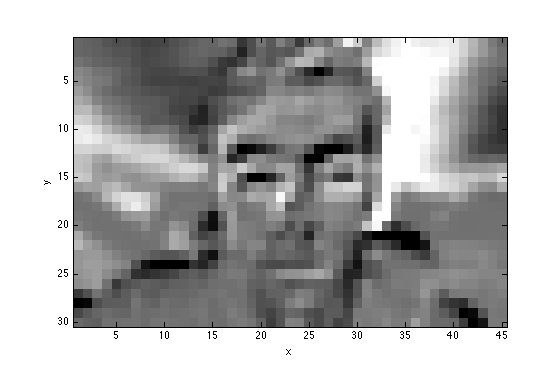
\includegraphics[width=\textwidth]{images/red_peak.png}
      \caption{At at a given time}
    \end{subfigure}
    \begin{subfigure}{.5\textwidth}
      \captionsetup{justification=centering}
      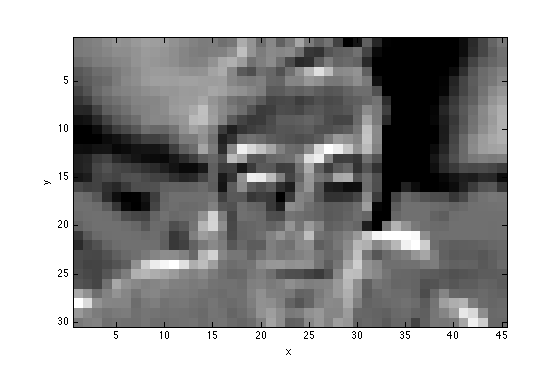
\includegraphics[width=\textwidth]{images/red_trough.png}
      \caption{Half a heartbeat period later}
    \end{subfigure}
    \captionsetup{justification=centering}
    \caption{Red channel of the EVM output, before recombining with the original video.}
  \end{figure}

  What is striking is that the output for these two frames seem like they are the same image with inverted colors. In fact, after processing, the whole video presents a 
  periodic color with a frequency that seems equal to the heartbeat. This does not happen with the data provided in the paper, where in a similar video only the person's face 
  changes color.

  Thus, while the EVM processing strikingly shows that it is possible to extract medically relevant data from a simple video, we also realized that processing had too many 
  unknown effects for us to get started by directly adding new layers on top of it. Thus we decided to start building from the ground up.

  Another question that arose from this visualization was whether or not it would be necessary to use some face detection tool in order to be able to look at the 'right' pixels (those with a heartbeat). We then realized we had actually had a wrong definition of our problem, up until then.

  What we are essentially trying to do is to get the same reading a pulse oximeter, but with a camera.
  An transmittance pulse oximeter measures the absorption of light by a thin layer of tissue through time. Because oxygenated and de-oxygenated hemoglobin do not absorb light at the same wavelength, this measure yields the blood's oxygen saturation, And by measuring the periodic change of absorbance caused by the pulse, the same measure also yields a heartbeat reading.

  Thus, we could see our experiment as one big pulse oximeter. The room is our light source, the camera our sensor. It happens that we have a video of a whole face, instead we could have only one pixel of the whole video and the concept would still work. With that different view, our problem changes, and the difficulty comes from the fact that we do not know much about either our light source or our sensors.

  %%%%%%%%%%%%%%%%%%%%%%%%%%%%%%%
\end{document}


